% ::setlocal makeprg=cd\ latex\ &&\ pdflatex\ -interaction=batchmode\ main.tex\ &&\ xdg-open\ main.pdf\ &&\ exit

\section{Equations of motion}
\label{cap2:sec:eq_of_motion}

Recalling the results of the previous chapter, we can rewrite equation
\eqref{cap1:eq:like_newton}, together with the
equations for $\phi$ and $t$ that came directly from the conservation of
angular momentum and energy per rest mass unit, respectively eq.
\eqref{cap1:eq:conserved_l} and \eqref{cap1:eq:conserved_e}.

\begin{subequations}
	\begin{align}[left = {\empheqlbrace}]
        &\frac{1}{2} \left(\dv{r}{\tau}\right)^2 = \mathcal E - V_{\rm eff} (r)
        \\
        &\dv{\phi}{\tau} = \frac{l}{r^2} \\
        &\dv{t}{\tau} = \frac{e}{1 - 2 M / r}
	\end{align}
\end{subequations}

Remembering that $\mathcal E = \frac{e^2 - 1}{2}$, and the expression for the
potential $V_{\rm eff}$ (eq. \eqref{cap1:eq:V_eff}), we can rewrite the system
as

\begin{subequations}
	\begin{align}[left = {\empheqlbrace}]
        &\dv{r}{\tau} = \pm \sqrt{2 \mathcal E - 2 \left(\frac{\ell^2}{2 r^2} 
        - \frac{M}{r} - \frac{M \ell^2}{r^3} \right)} \label{cap2:eq:radial_eq} \\
        &\dv{\phi}{\tau} = \frac{l}{r^2} \label{cap2:eq:angular_eq} \\
        &\dv{t}{\tau} = \sqrt{2 \mathcal E + 1}\left(1 - \frac{2 M}{r} \right)^{-1}
	\end{align}
\label{cap2:eq:eq_of_motion}
\end{subequations}

To avoid numerical problems, we will keep geometrized units and express
everything in unit of the \Sh radius $r_s = 2 M$:

\begin{equation}
    r = r_s \hat r \quad \quad
    \tau = r_s \hat \tau \quad \quad
    t = r_s \hat t \quad \quad
    \ell = r_s \hat \ell \quad \quad
\end{equation}

The system of equations \eqref{cap2:eq:eq_of_motion} can be rewritten as

\begin{subequations}
    \begin{align}[left = {\empheqlbrace}]
        &\dv{\hat r}{\hat \tau} = \pm \sqrt{2 \mathcal E
        - \left(\frac{\hat \ell^2}{2 \hat r^2} - \frac{1}{2 \hat r}
        - \frac{\hat \ell^2}{2 \hat r^3} \right)}
        \label{cap2:eq:radial_eq_dimless} \\
        &\dv{\phi}{\hat \tau} = \frac{\hat \ell}{\hat r^2}
        \label{cap2:eq:angular_eq_dimless} \\
        &\dv{t}{\hat \tau} = \sqrt{2 \mathcal E + 1}
        \left(\frac{\hat r}{\hat r - 1}\right) \label{cap2:eq:time_eq_dimless}
    \end{align}
    \label{cap2:eq:eq_of_motion_dimless}
\end{subequations}

The condition on the angular momentum $\ell$ for the existence of a stable
orbits $\ell > \sqrt{12} M$ becomes $\hat \ell > \sqrt{3}$.
The stationary points of $V_{\rm eff}$ from eq. \eqref{cap1:eq:V_eff} are

\begin{subequations}
    \begin{align}
        \hat r_{1 / 2} &= \hat \ell^2
        \left(1 \pm \sqrt{1 - \frac{3}{\hat \ell^2}} \right)\\
        \hat r_{\rm ISCO} &= 3
    \end{align}
\end{subequations}

\begin{figure}[h]
    \centering
    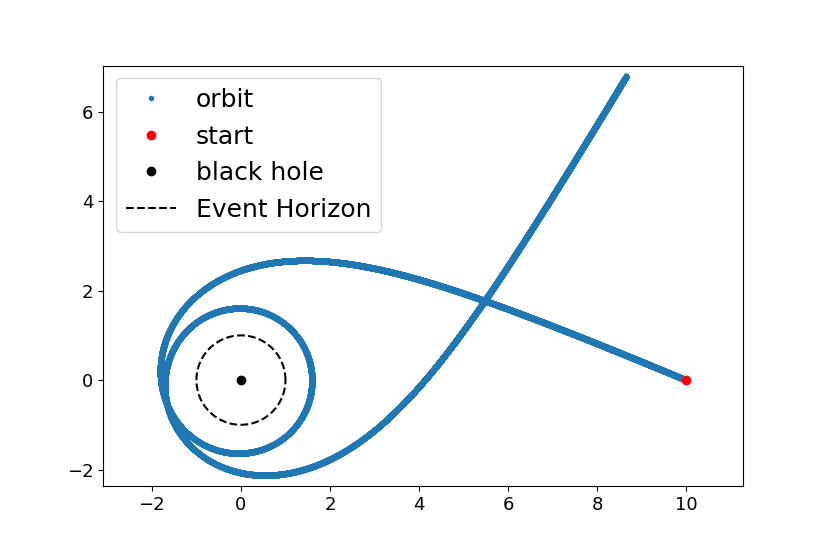
\includegraphics[width=0.7\textwidth]{Figures/chapter2/cool.png}
    \caption{Unbound orbits spanning an angle greater than $2 \pi$ before going
    to infinity.}
    \label{cap2:fig:V_eff}
\end{figure}
